% status: 100
% chapter: Amazon

\makeatletter
\newcommand{\verbatimfont}[1]{\def\verbatim@font{#1}}%
\makeatother

\verbatimfont{\footnotesize}

\title{Interacting With Data Services on AWS}

\author{Scott Steinbruegge}
\affiliation{%
  \institution{Indiana University}
  \city{Bloomington} 
  \state{IN} 
  \postcode{47408}
  \country{USA}}
\email{srsteinb@iu.edu}

% The default list of authors is too long for headers}
\renewcommand{\shortauthors}{S. Steinbruegge}

\begin{abstract}
Amazon Web Services provides a wide variety of data related services that 
allow a user to immediately start working on utilizing and interpreting their 
data instead of trying to obtain or provision their own hardware beforehand. 
By using a data set that contains Medicare hospital patient survey 
information, we showcase how REST APIs can be used to directly interact with 
multiple AWS services that are used specifically for data related use cases. 
We provide some examples of how to interact with these services 
through the AWS Management Console, but the AWS Python SDK called Boto is the 
main method used in our project in order to be able to work programmatically 
with the Amazon APIs. We start with presenting how to get raw data onto the 
AWS platform directly from the web and landing that data in S3 for use by 
other AWS services such as Data Pipeline, RDS, Redshift, DynamoDB and Athena. 
Along the way we provide explanations and hands on coding examples for each 
service in order to gain insight into how to effectively interact with AWS 
while performing a variety of data related tasks. 
\end{abstract}

\keywords{hid-sp18-521, Amazon, AWS, Swagger, AWS Data Services}

\maketitle

\section{User Interactions With AWS}

Between the AWS Management Console, SDKs (software development kits) and AWS 
CLI (command line interface), AWS provides multiple ways to interact with 
their services. While some of the work we perform is done through the 
Management Console, the majority of it is performed by the Python SDK for 
AWS named Boto. Using one of the AWS SDKs allows developers to be able to 
write their own software that interacts directly with AWS services through 
their own set of APIs. There are two levels of APIs that AWS provides, 
resource APIs and client APIs. The resource APIs provide an object-oriented 
interface to the services which expose multiple attributes and methods per 
service at a higher level than the lower level client API 
calls~\cite{hid-sp18-521-BotoResources}. Client APIs, also called low-level 
APIs, provide methods that map one-to-one with the service APIs. No level of 
abstraction is provided by the client APIs, the developer needs to explicitly 
provide all information about the targeted resource for every client API 
call~\cite{hid-sp18-521-BotoClients}. When available, the resource APIs are 
preferred since they abstract the majority of the backend details away from 
the developer and they can focus on interacting directly with the service 
using the necessary parameters. Boto also provides the ability to use 
waiters, which allow for polling the status of specific AWS resources within 
your code. An example of when a waiter could be used is when you run code 
trying to provision a new resource and moving onto the next step cannot be 
done until that new resource has been setup successfully. Using the waiter 
would allow your code to continuously poll the status of that dependent 
service~\cite{hid-sp18-521-pythonsdk}.

\section{Utilizing Data Services on AWS}

To provide examples on how to work with data on several AWS platforms, we 
utilized a sample data set from the Medicare data website that contains ``a 
list of hospital ratings for the Hospital Consumer Assessment of Healthcare 
Providers and Systems (HCAHPS). HCAHPS is a national, standardized survey of 
hospital patients about their experiences during a recent inpatient hospital 
stay~\cite{hid-sp18-521-MedicareData}.'' This data set was provided in both 
CSV and JSON format which allowed us to choose which data format was best 
suited for the specific AWS service we worked on. Preliminary data analysis 
on the raw file showed 23 columns and approximately 264,000 rows of data. 
For each AWS service we chose to work with, we attempted to perform a 
different type of analysis on this data in order to show how a user would be 
able to gain insights from data residing within different AWS locations. 

The AWS Management Console was used during the initial setup of our project 
environment in order to provision certain services. We felt it would be best 
to keep our costs low for this project by not exposing the ability to 
provision high cost AWS services through a REST API. Interacting with each of 
these services though was still done through Boto in order to keep the 
majority of the tasks done in programmatic fashion. At a high level, our 
project uses multiple Swagger REST APIs which then call Python functions that 
use Boto and additional libraries to interact directly with AWS service 
specific APIs to perform different types of data interactions. In order to be 
able to programmatically interact with AWS, an IAM user needed to be created 
and permissions had to be assigned for all of the AWS services it would be 
interacting with.  

An IAM user is a login created on the AWS platform that can then be used to 
access multiple AWS services based on the permissions assigned to 
it~\cite{hid-sp18-521-IAMOverview}. This user creation was accomplished 
through the AWS Management Console so that access keys could then be easily 
obtained upon new user creation which then allowed this user to have 
programmatic access to AWS services~\cite{hid-sp18-521-IAMkeys}. In order to 
create our IAM user, we logged into the console and selected IAM from the 
services menu. On the left side of the next screen we then selected the menu 
option users which took us to the user information page where we selected the 
add user button. We then chose the user name i524user and selected only the 
check box that allows the user to have programmatic access through an access 
key ID and secret access key and then selected the permissions button to 
proceed. On the permissions page we then chose to attach existing policies to 
this new user in order to grant it permissions to the AWS services it would be 
using. During initial user creation only one existing policy can be attached, 
so we selected the AmazonS3FullAccess policy which grants full access to all 
S3 buckets for the entire AWS account the IAM user exists under. While 
permissions could have been granted more granular, for this project, this 
policy would do what we needed. After the existing policy was selected, we 
clicked the review button which took us to a page showing an overview of the 
user options. We were satisfied with our selections and clicked create user. 
The next page showed the access key ID and secret access key that we would 
need to save in a secure location in order to use within our Python code later 
on. The secret access key information is only presented once after the user 
has been created. If it is lost it cannot be retrieved and a new set of keys 
would need to be generated for this user~\cite{hid-sp18-521-IAMkeys}. We were 
then able to go back to the user menu and select the name of the new user we 
created to bring up the permissions page. From there we selected the add 
permissions button and attached existing policies like we did during the 
initial user creation for the remaining AWS services we would be working with 
later on: Data Pipeline, RDS, Redshift, DynamoDB and Athena. Now that we had 
our user created and the proper permissions assigned to it, we were then able 
to get started on setting up and interacting with each of the AWS data 
services. The final list of policies assigned to our user are displayed in
Figure~\ref{f:iam}.

\begin{figure}[!ht]
  \centering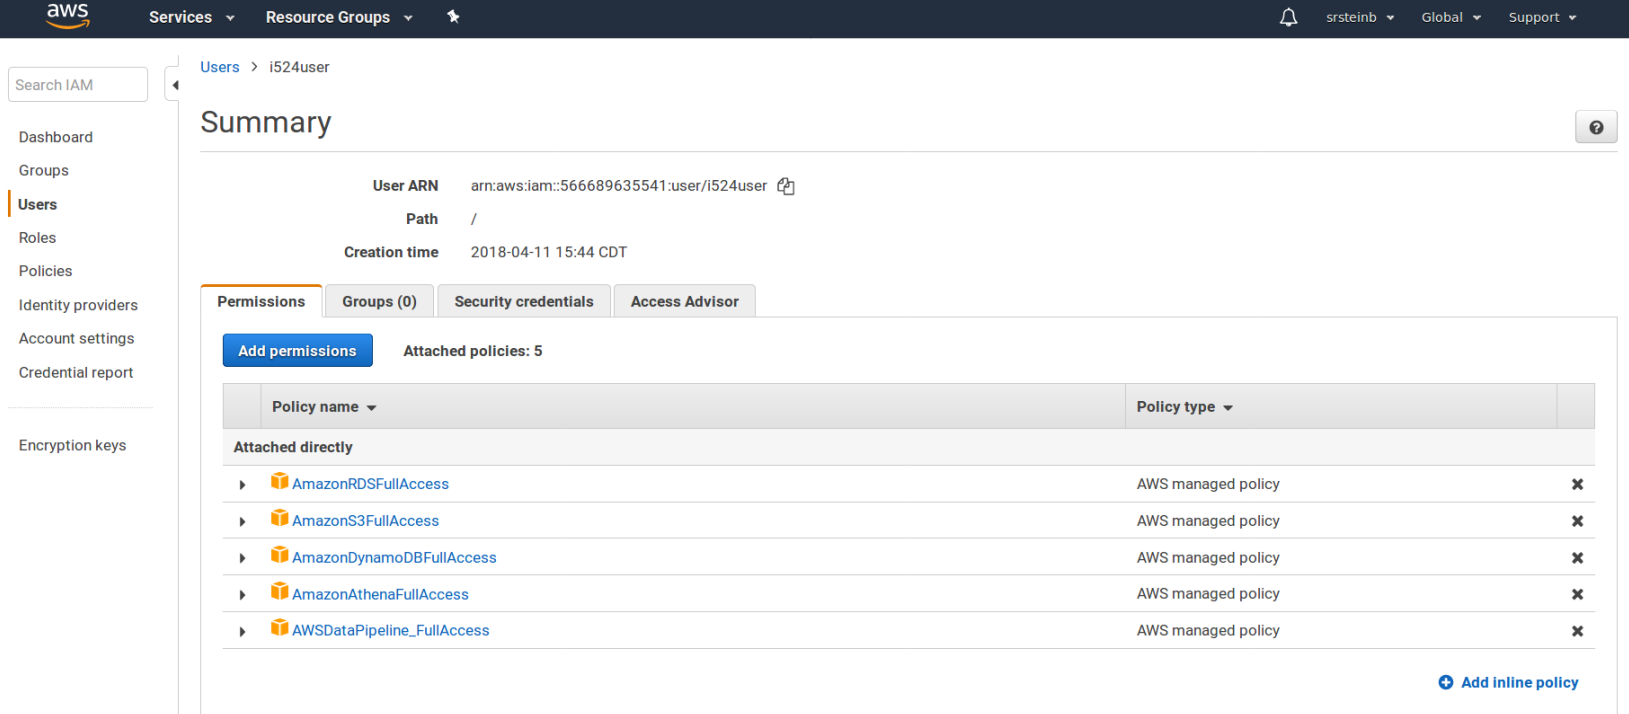
\includegraphics[width=\columnwidth]{images/iam.png}
  \caption{IAM user permissions}\label{f:iam}
\end{figure}

Programmatically interacting with services on AWS requires the code to utilize 
both the access key ID and secret access key generated upon IAM user creation. 
Along with these keys, several other data services require that a separate 
user login be created directly within the service itself, such as Amazon RDS 
and Redshift. In order to be able to store and reuse the credentials needed 
for this project, we stored these values in a YAML configuration file. Using 
the YAML Python library we could then import the YAML configuration file into 
our Python code, store it in a list variable and then assign user names and 
passwords to variables for each service needing credentials. The majority of 
connections to the AWS services utilized need only the IAM access keys but 
connecting to the MySQL instance on RDS and the Redshift database both 
required separate user names and passwords. We chose to store the access key 
ID in the k1 variable and the secret access key in the k2 variable to better 
mask what they really are since it is best to keep these keys secure as 
possible~\cite{hid-sp18-521-IAMkeys}. The Python code used to pull connection
information from the YAML file is shown in Figure~\ref{f:yaml}. 

\begin{figure}[!ht]
\begin{verbatim}
with open(os.path.expanduser(
``~/.cloudmesh/configuration-awsdataservices.yml''), 'r') as ymlfile:

config = yaml.load(ymlfile)

mysql_user = config['cloudmesh']
['aws-data-services']['mysql']['user']['name']

mysql_password = config['cloudmesh']
['aws-data-services']['mysql']['user']['password']

redshift_user = config['cloudmesh']
['aws-data-services']['redshift']['user']['name']

redshift_password = config['cloudmesh']
['aws-data-services']['redshift']['user']['password']

k1 = config['cloudmesh']['aws-data-services']['misc']['k1']

k2 = config['cloudmesh']['aws-data-services']['misc']['k2']
\end{verbatim}
\caption{Python code to import YAML configuration settings}\label{f:yaml}
\end{figure} 

\subsection{S3}

Once our IAM user was created, we were ready to start ingesting our raw data 
into AWS. As a starting point, we chose to land our raw CSV and JSON files in 
S3. ``Amazon S3 stores data as objects within resources called buckets. You 
can store as many objects as you want within a bucket, and write, read, and 
delete objects in your bucket~\cite{hid-sp18-521-S3features}.'' We created our 
bucket through the AWS Management Console by browsing the services menu and 
selecting S3 from the services list. From there we selected the create bucket 
button, entered a bucket name of hid-sp18-521 and left all of the other 
options to what they were defaulted to since our IAM user has full access to 
S3 for this project and then created the bucket. 

With our S3 bucket in place, we were then ready to start writing our Python 
code to interact with the AWS services. The first function we implemented was 
to pull the raw Medicare data files in both CSV and JSON format directly from 
the web into our S3 bucket. This was accomplished by using the Python library 
smart open. This library could be used to stream large data files to and from 
a variety of data sources including S3 and HTTP~\cite{hid-sp18-521-smartopen}. 
To connect to the S3 bucket we had to specify the destination file and bucket 
name as well as the access key ID and secret access key of our IAM user. A for 
loop is then used to import all of the rows in the raw file directly from the 
HTTP location where the file is stored and writes it to the S3 destination 
file provided. If the copy was performed successfully, the response returned 
is the total size of the file that was written into S3. Code to perform this 
task for both the CSV and JSON import into S3 were exactly the same except for 
the file extension. Both of these functions could be rerun as needed and the 
S3 file would just get overwritten if it already existed. The Python code used
to import the raw data files into S3 is shown in Figure~\ref{f:rawdata}. 

\begin{figure}[!ht]
\begin{verbatim}
with smart_open.smart_open('s3://' + k1 + ':' + k2 
+'@hid-sp18-521/PatientSurveyData.csv', 'wb') as fout:

   for line in smart_open.smart_open('https://data.medicare.gov/resource/
   rmgi-5fhi.csv'):
       
      response = fout.write(line + '\n')

return response
\end{verbatim}
\caption{Python code to import raw data files into S3}\label{f:rawdata}
\end{figure} 

Once the raw data was in place in S3, we wanted to verify that the files we 
copied actually existed in our S3 bucket. To do this, we connected to the S3 
resource API by assigning a variable to the S3 resource object and provided 
the parameters for AWS service name, region and access keys. The S3 resource 
API contained the class named bucket which was used to specify which bucket 
name we were interested in using~\cite{hid-sp18-521-boto-bucket}. We were then 
able to setup a for loop to use the bucket class method called object to get 
the names of all files located within our S3 bucket and append them to a list 
variable. This list variable would then be returned to our API to show all of 
the names of the files located within our project specific bucket. The Python 
code used to list all files located in the S3 bucket is shown in 
Figure~\ref{f:s3bucket}.

\begin{figure}[!ht]
\begin{verbatim}
file_names = []

s3 = boto3.resource('s3', region_name='us-east-1'
, aws_access_key_id=k1, aws_secret_access_key=k2)

bucket = s3.Bucket('hid-sp18-521')

for object in bucket.objects.all():
   file_names.append(object.key)

return file_names
\end{verbatim}
\caption{Python code to show all files located in S3 bucket}\label{f:s3bucket}
\end{figure} 

\subsection{RDS}

Now that our raw data files were landed on the AWS platform within S3, we then 
had more options to be able to extract, transform and load this data to 
various other AWS data services. Our next task was to import our CSV data 
file into an Amazon RDS database. Before importing the S3 data an RDS instance 
needed to be provisioned. RDS is a ``managed relational database service which 
offers six database engine choices and allows users to setup, operate and 
scale relational databases within the AWS 
cloud~\cite{hid-sp18-521-rds-mysql}.'' The six database platforms RDS works 
with are Amazon Aurora, MySQL, MariaDB, Oracle, SQL Server, and PostgreSQL. 
For the purposes of this project, we chose to implement a MySQL instance since 
it fell within our AWS account free usage tier. When we refer to the term 
instance in regards to working with RDS, it can be thought of as a database 
server, which would then contain multiple databases within that 
instance~\cite{hid-sp18-521-rds-mysql}. Since exposing access to create RDS 
instances was not something we wanted to do in order to make sure our costs 
for the project remained low, we decided to perform a one-time setup an RDS 
MySQL instance through the AWS Management Console.  

To access the RDS console, search to the RDS service in the AWS services list 
which brings up the RDS dashboard. The dash displays information about the 
existing RDS resources that are currently allocated. Since we have not created 
any RDS instances yet, we selected the instances menu on the left side of the 
dashboard which took use to the page where we could then select the launch DB 
instance button to get started. The first choice to make was which engine to 
use. At the bottom of this screen there was a checkbox we selected that only 
showed the engine options available for free tier usage. We chose MySQL since 
it is a very popular open source database engine and clicked the next button. 
The following page asked us to specify our instance specifications and 
settings. Due to free tier restrictions, we did not change any of the default 
instance specifications and were just able to provide a name for our instance, 
iu-sp18, as well as a master user name and password. Moving onto the next 
page, we chose to leave all of the defaults in place for the network and 
security options and made sure that the option was selected to setup the 
instance to be publicly accessible. Under database options we could then 
select a default database name to be created on the instance, which was named 
I524, and then left the remaining options on this page in place as their 
defaults since they served our needs to the project use case. We were then 
able to select the launch DB instance button at the bottom of the screen and 
AWS started the provisioning of the MySQL instance which took about 5 to 10 
minutes total to come online and ready for 
connections~\cite{hid-sp18-521-rds-mysql}. 

Once the instance was running, it was time to log into the instance using the 
master user and password we setup upon creation in order to create an 
additional user login and the table we would use to import our data into. 
Interacting with a database residing on RDS is accomplished the same way a 
user would connect to an on-premise database server. There is a free GUI based 
application provided by MySQL named MySQL Workbench that we used to perform 
our first set of interactions with the instance. In order to connect to the 
instance, we needed the name of the endpoint and port number, which could be 
found under the instances menu on the RDS dashboard page by clicking the name 
of the instance in the list. About half way down the instance details page in 
the connect section was the endpoint and port number, which are always needed 
when setting up any connections to this instance, either through a GUI 
application or programmatically. Once we had all of the connection information 
needed, we were able to successfully login to the RDS instance through MySQL 
Workbench. From here, we executed standard SQL statements against the I524 
database to create a new database user, named IUuser, which we would use for 
programmatically connecting through our APIs and created the empty table 
schema named PatientSurveyData that would contain the CSV data imported 
from S3~\cite{hid-sp18-521-rds-mysql}. The location of the RDS endpoint and
port number within the AWS Management Console is shown in Figure~\ref{f:rds}.

\begin{figure}[!ht]
  \centering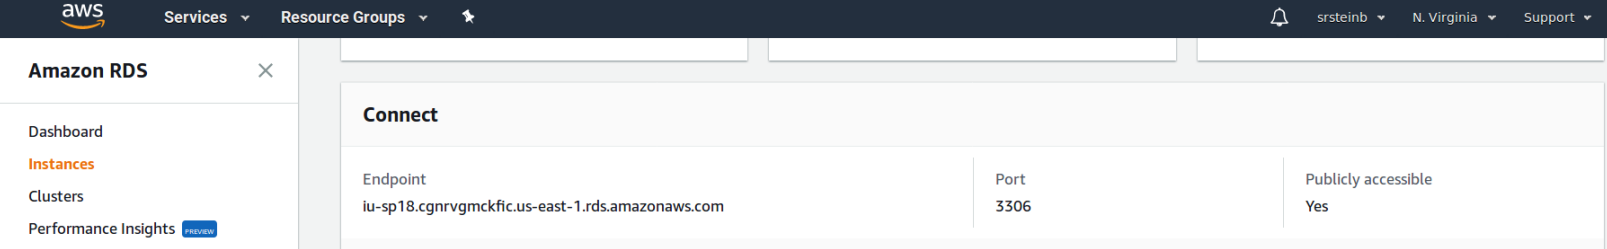
\includegraphics[width=\columnwidth]{images/rds.png}
  \caption{RDS server information}\label{f:rds}
\end{figure} 

\subsection{Data Pipeline}

In order to get the data into our RDS instance from S3, we utilized AWS Data 
Pipeline, which ``is a web service that you can use to automate the movement 
and transformation of data~\cite{hid-sp18-521-whatisdatapipeline}.'' In 
broader IT terminology, it could be considered an AWS specific extract, 
transform, load (ETL) tool. It consists of multiple pieces of data driven 
workflows that are dependent upon successful competition of one another. 
The user can specify parameters to interact with transformations run against 
various sets of data and related services and Data Pipeline will handle the 
application of this logic. Data Pipeline consists of three main components, 
the first being a pipeline definition, which specifies the logic to applied 
during data transformations and management. Next is the pipeline itself, which 
handles the scheduling and execution of the defined tasks by creating an EC2 
instance to perform the work specified by the pipeline definition. Lastly, 
the task runner handling the polling between tasks within the pipeline and 
performs those tasks as needed. Task runner is also installed and set to run 
automatically on all resources used by your pipeline 
definition~\cite{hid-sp18-521-whatisdatapipeline}. 

The AWS Management Console provides a web-based interface that allowed us to 
create and interact with pipelines. As we were novices with the service, 
this was the best place to start working in order to gain an understanding on 
how to properly setup and execute a pipeline. To start creating our pipeline 
to import data from our S3 bucket in the MySQL RDS database, we had to 
navigate to the AWS Data Pipeline service listed under the services menu on 
the main dashboard of the AWS Management Console. From there, since we had yet 
to create any pipelines, it presented an intro screen and we selected the 
button get started now to proceed. The next page is where we specified the 
pipelines name and source. Under the source options, there were options to 
build using a template, import a definition or build using Architect. Using 
the template option for our use case made the most sense, especially since it 
provided a specific load S3 data into RDS MySQL table template to build our 
pipeline from. Once the template was selected, we were then prompted to 
provide information related to the source S3 file we wanted to utilize as well 
the connection information and location of the MySQL RDS destination we wanted 
to import into. For S3, only the file path was needed, but for RDS we needed 
to supply the RDS instance name, user name and password to connect with, the 
standard SQL based insert statement we'd use to insert data in our MySQL table 
we created earlier named PatientSurveyData and an optional statement which we 
utilized to clear out all of the data in the existing MySQL table before we 
imported the data from the S3 file~\cite{hid-sp18-521-datapipelinestarting}.

After specifying all of these pipeline parameters, we then scrolled down to 
the scheduling section where we chose to run our pipeline on activation only, 
meaning we didn't want it to run on any set schedule, only whenever it was 
manually started. The rest of the options below this we left as default and 
proceeded to the bottom of the page and clicked the activate button to create 
and start our pipeline. The pipeline creation did not produce any errors and 
we were taken to a screen where we could monitor the execution details of our 
pipeline. By using the refresh button on the right side of the screen we were 
able to track the status of each step within the pipeline and determine where 
the process was currently at. Our pipeline consistent of two components, the 
first provisioned the EC2 instance which performed the execution of the SQL 
code against our RDS database to delete data from the existing table and 
create it if it does not already exist. Upon successful completion of that 
step, the pipeline then starts a component to load the data from S3 into the 
RDS database which is executed from the same EC2 instance that was created in 
step one. Once both components completed with a status of successful, we were 
ready to query the MySQL table and interact with the Medicare data within a 
relational database in the AWS cloud~\cite{hid-sp18-521-datapipelinestarting}.
Figure~\ref{f:datapipeline} shows the layout of how the data pipeline looks 
within Architect as well as the parameters we specified upon creation of the 
pipeline.  

\begin{figure}[!ht]
  \centering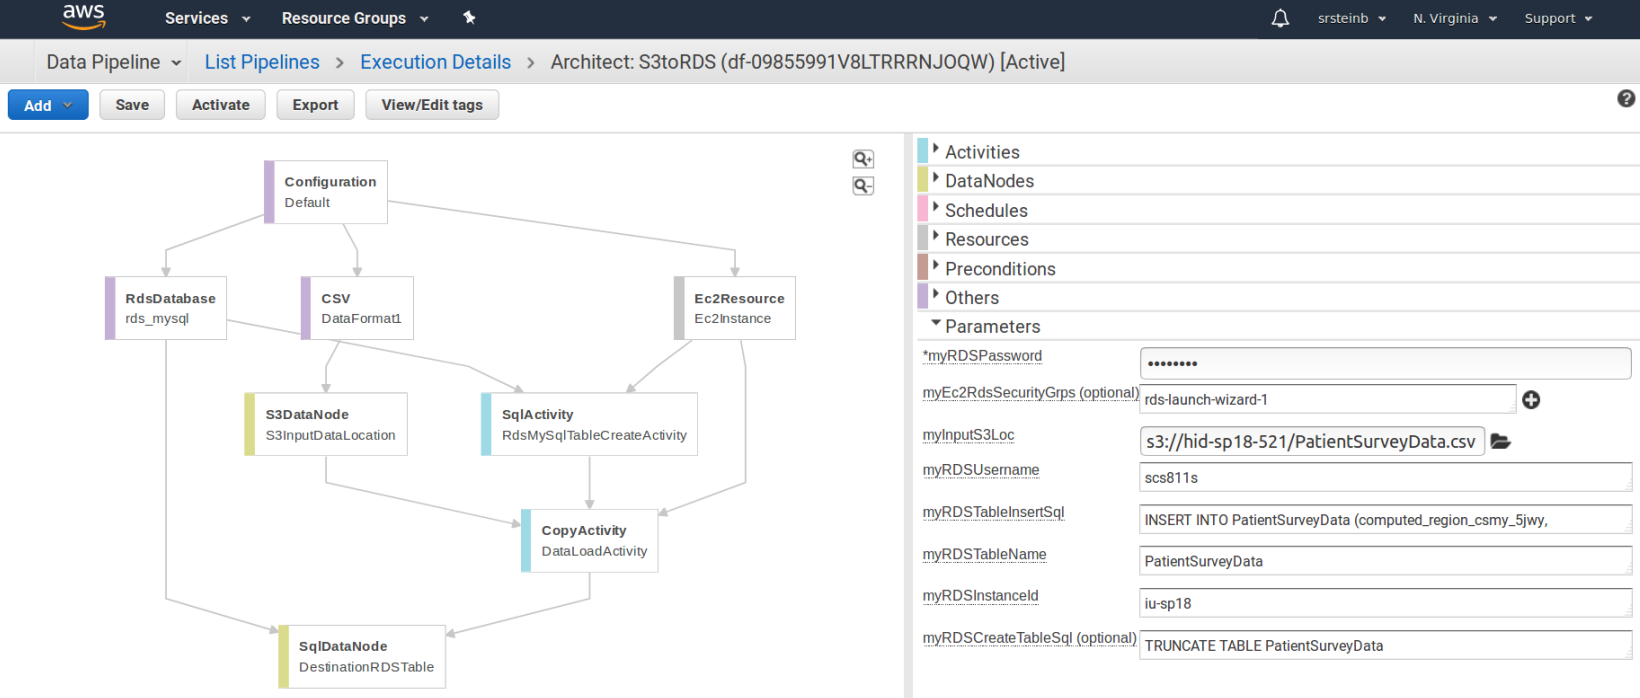
\includegraphics[width=\columnwidth]{images/datapipeline.png}
  \caption{Data Pipeline layout and parameters}\label{f:datapipeline}
\end{figure} 

With pipeline in place and tested to work successfully, we wanted to implement 
functionality within our code that would allow a user to both activate and 
check the execution status of our data pipeline on demand.  Boto would allow 
us to accomplish these tasks through our Python code by utilizing the Data 
Pipeline API. We assigned a variable to the client API connection for data 
pipeline by providing the resource name, region, access key ID and secret 
access key in the same manner we did for the S3 code. We could then use the 
activate pipeline function and pass in the pipeline ID, which can be retrieved 
from the list pipelines screen on the Data Pipeline page in AWS Management 
Console. This code then allowed us to activate our pipeline through an API 
call whenever we wanted. A similar approach was taken when pulling the status 
of an existing data pipeline. But for this one we needed to use the 
describe pipelines method and return the string value of a key named 
@pipelineState from the list of pipeline descriptions for this pipeline in 
order to present the current runtime status. So now we were able to monitor 
the status of the pipeline job we were just able to start within another 
API~\cite{hid-sp18-521-botodatapipeline}. The Python code used to both start
the pipeline and check the status of the pipeline is shown in 
Figure~\ref{f:datapipelinecode}. 

\begin{figure}[!ht]
\begin{verbatim}
pipeline = boto3.client('datapipeline', region_name='us-east-1', 
aws_access_key_id=k1, aws_secret_access_key=k2)

response = pipeline.activate_pipeline(pipelineId='df-09855991V8LTRRRNJOQW')

return response
---
pipeline = boto3.client('datapipeline', region_name='us-east-1', 
aws_access_key_id=k1, aws_secret_access_key=k2)

pipeline_status = 
        pipeline.describe_pipelines(pipelineIds=['df-09855991V8LTRRRNJOQW'])

fields = pipeline_status['pipelineDescriptionList'][0]['fields']

for field in fields:
   if field['key'] == '@pipelineState':
      return field['stringValue']
\end{verbatim}
\caption{Python code to start and return status of data pipeline}
\label{f:datapipelinecode}
\end{figure} 

Once the pipeline execution was in place within our code, we then felt 
comfortable enough to develop an API to run a query against the data we 
imported in our MySQL RDS database. When programmatically interacting with an 
RDS database, an Amazon specific API is not necessary. We could use any 
library that we'd normally use to connect to a MySQL database whether it was 
cloud based or not. PyMySQL was the library we chose to utilize for this 
project. After importing the library into our code, we were then able to 
define a function that first assigned a variable to a MySQL connection object 
by providing the host name, which was the endpoint name listed within RDS, a 
user name and password, which was stored in the variables imported from the 
YAML configuration files, a database name, charset and cursor class, which we 
specified to return any results as a dictionary data type. We were then able 
to assign this connection object to a cursor object which would allow us to 
further interact with the MySQL database. To query a specific subset of data 
we were interested in, we developed a SQL select query to return all of the 
rows from the table where the star rating for the hospitals was listed was 
five. We allowed the function to accept a parameter of starRating and used in 
within the SQL statements where clause in order to filter the data we were 
interested in returning. The SQL statement was then run by calling the execute 
method using the SQL query variable and starRating parameter as arguments. 
The fetchall method was then invoked to collect all of the rows returned in 
the results and return them to our API for presentation to the 
user~\cite{hid-sp18-521-pymysql}. The Python code used to query the MySQL RDS
database is shown in Figure~\ref{f:rdscode}. 

\begin{figure}[!ht]
\begin{verbatim}
connection = pymysql.connect(
host='iu-sp18.cgnrvgmckfic.us-east-1.rds.amazonaws.com',
user=mysql_user,
password=mysql_password,
db='I524',
charset='utf8mb4',
cursorclass=pymysql.cursors.DictCursor)

cursor = connection.cursor()
sql = ``SELECT * FROM PatientSurveyData WHERE patient_survey_star_rating = %s''

cursor.execute(sql, (starRating))
result = cursor.fetchall()
return result
\end{verbatim}
\caption{Python code to query the MySQL RDS database}
\label{f:rdscode}
\end{figure} 

\subsection{DynamoDB}

Since we had access to our data set in JSON format, we wanted to explore the 
idea of being able to ingest this raw data into a NoSQL database for 
additional analysis. DynamoDB is a fully managed database service that 
supports document and key-value storage models. There is no need to create 
or manage individual databases, all tables created and utilized will be 
placed in whatever region is specified upon table creation. Like RDS, the 
database software and hardware provisioning are handled by AWS, allowing 
to user to focus solely on managing their data. DynamoDB runs only on SSD 
drives in order to provide low-latency response times for all database 
operations on the platform. The data model within DynamoDB consists of 
tables, items and attributes. Tables are a collection of items and can store 
an infinite number of items. In relational database terms, an item can be 
thought of a row of data, which consists of a primary key and any number of 
additional attributes, there is no limit. An attribute is a specific element 
of data within an item that consists of an attribute name and value. As the 
platform is schema less, each item does not need to have the same number or 
name of attributes. Every table created must have a primary key assigned which 
can consist of either a single attribute or multiple attributes and the 
primary key must exist for every item. The only limitation on an item is that 
it must be under 400 KB in size. As there is nothing to setup ahead of time 
other than allowing our IAM user access to use the DynamoDB service, we could 
jump right into using Boto for our interacts with this database 
platform~\cite{hid-sp18-521-dynamodbfaq}. 

Creating a DynamoDB table was our first step which we were able to do within 
Boto by using the DynamoDB resource API. To creation a service connection, we 
needed to pass in the region name, access key ID and secret access key. From 
there, we were then able to call the create table method and provide several 
required arguments. The table name was provided as well as the key schema, 
which identifies what attributes would be the primary key and the key type 
for each attribute used. Our data had a key in place already named provider ID 
which was used as the primary key for the DynamoDB table as well. There were 
two options for key type, hash or range. A hash key, also called a partition 
key, which is used to handle distribution of the data across multiple 
partitions, and a range key, also called a sort key, which indicates how the 
data stored in DynamoDB will be sorted. For single attribute primary key, a 
hash key needed to be used as the key type. We also needed to supply the 
definitions of the attributes we chose to use as our key. We specified this 
as provider ID and assigned it a data type of string. The last argument we 
needed to supply in order to create a table was provisioned throughput, which 
was the amount of read and write activity the table could 
support~\cite{hid-sp18-521-dynamodbfaq}.  

If the table we created was in a highly transactional environment we would 
need to take time to consider how to calculate what values we would need to 
set the read and write capacity units to. These throughput settings are used 
to take into account how many systems resources would need to be reserved in 
order to meet the I/O requirements. The values are submitted in terms of 
capacity units, or amount of data the table needed to handle per second. 
To be able to calculate the amount of capacity units we needed to determine 
our data sets average item, or row, size. By taking the total file size of 
our raw JSON file, which was 937 KB and dividing that by the total number of 
rows objects within the file, which was 1000, to get an average item size of 
approximately 1 MB. ``One read capacity unit represents one strongly 
consistent read per second, or two eventually consistent reads per second, 
for an item up to 4 KB in size. If you need to read an item that is larger 
than 4 KB, DynamoDB will need to consume additional read capacity 
units~\cite{hid-sp18-521-dynamodbreadwrite}.'' Same concept applies for write 
capacity units, except it is for an item up to 1 KB in size. Since our item 
size and I/O footprint was low for our project use case, we decided to use 
just 5 read and write capacity units to keep our costs down. With all of the 
required arguments gathered, we could now submit the resource API call to AWS 
to create a new table. Creation of the table itself took several minutes and 
once it was ready to use we were then able to start inserting data into our
new DynamoDB table~\cite{hid-sp18-521-dynamodbreadwrite}. The Python code used 
to create the DynamoDB table is is shown in Figure~\ref{f:dynacreatetable}. 

\begin{figure}[!ht]
\begin{verbatim}
dynamodb = boto3.client('dynamodb', region_name='us-east-1', 
aws_access_key_id=k1, aws_secret_access_key=k2)

response = dynamodb.create_table
   (TableName='PatientSurveyData',
    KeySchema=[{'AttributeName': 'provider_id', 'KeyType': 'HASH'}, ],
    AttributeDefinitions=[{'AttributeName': 'provider_id', 
      'AttributeType': 'S'}],
    ProvisionedThroughput={'ReadCapacityUnits': 5, 'WriteCapacityUnits': 5},
)

return response
\end{verbatim}
\caption{Python code to create the DynamoDB table}
\label{f:dynacreatetable}
\end{figure} 

The resource API for DynamoDB provided a class named table which allowed us to 
execute table specific functions by providing a table name argument. We also 
utilized the Python library urlib to import the JSON file from its source on 
the web directly into our DynamoDB table~\cite{hid-sp18-521-urllib}. The 
urlopen function was called against the HTTP path of the JSON file and stored 
into a variable. This variable containing the file data could then be read 
into a loading function provided by the Python JSON library to convert the 
data into proper JSON format that could be accepted by the DynamoDB put item 
method~\cite{hid-sp18-521-botodynamodb}. The Python code used to insert into 
the DynamoDB table is is shown in Figure~\ref{f:dynainserttable}. 
 
\begin{figure}[!ht]
\begin{verbatim}
dynamodb = boto3.resource('dynamodb', region_name='us-east-1', 
aws_access_key_id=k1, aws_secret_access_key=k2)

table = dynamodb.Table('PatientSurveyData')

url = ``https://data.medicare.gov/resource/rmgi-5fhi.json''

response = urllib.urlopen(url)

data = json.loads(response.read(), parse_float=decimal.Decimal)

for row in data:
   response = table.put_item(Item=row)

return response
\end{verbatim}
\caption{Python code to insert into the DynamoDB table}
\label{f:dynainserttable}
\end{figure} 


Upon successful insert of the data into our DynamoDB table, we could then 
write code to pull back data from the database using the table class from 
the resource API. Normally we would just want to query this table for the 
information needed, but DynamoDB has different requirement for using specific 
query functionality than a normal relational database engine does. A query can 
only be used when a table has a composite primary key, which consists of both 
a partition key and sort key or has a secondary index that contains a 
composite key. Since our example utilized a simple primary key consisting of 
only a partition key with no additional indexes created on the table, we 
needed to use the scan function in order to access the data. The main 
different between a query and scan is that the scan always searches through 
the entire table to find the data and then filters out the necessary data 
based on the filter expressions provided. Using a query removes the additional 
step of having to filter out the data and can directly access the data 
required based on either the composite key or indexes that were created on the 
table, making it a better choice if faster response times are needed for 
larger sets of data. Scan worked for our specific needs in this project and 
worked similarly to query code wise in that the main required parameters 
needed to retrieve data were table name and filter 
expression~\cite{hid-sp18-521-botodynamodb}. The DynamoDB API provides a set 
of conditions that can be used to pull back data based on whatever criteria 
and attributes you specify through the filter expression parameter. With our 
sample dataset, we were interested in returning all of the hospitals from the 
patient survey data that were located in the state of Missouri. To do this, we 
utilized the eq condition run against the attribute state in order to return 
all items in the state of MO~\cite{hid-sp18-521-boto-dynamodbconditions}.  
The Python code used to scan data from the DynamoDB table is is shown in 
Figure~\ref{f:dynascantable}. 

\begin{figure}[!ht]
\begin{verbatim}
dynamodb = boto3.resource('dynamodb', region_name='us-east-1', 
aws_access_key_id=k1, aws_secret_access_key=k2)

table = dynamodb.Table('PatientSurveyData')

response = table.scan(FilterExpression=Attr('state').eq('MO'))

items = response['Items']

return items
\end{verbatim}
\caption{Python code to scan data from the DynamoDB table}
\label{f:dynascantable}
\end{figure} 

Using either the resource or client API, we could then delete the DynamoDB 
table once it was no longer needed. It was equally simple to delete a table 
using either API, so we wanted to show how the client API could be used to 
delete a table. It's used similar to other services in that we provide the 
service name, region and key parameters to allow us to connect to the service 
and then we could run the delete table method and just supply the table name 
as a parameter in order to delete our table~\cite{hid-sp18-521-botodynamodb}.
The Python code used to delete the DynamoDB table is is shown in 
Figure~\ref{f:dynadeletetable}. 

\begin{figure}[!ht]
\begin{verbatim}
dynamodb = boto3.client('dynamodb', region_name='us-east-1', 
aws_access_key_id=k1, aws_secret_access_key=k2)

response = dynamodb.delete_table(TableName='PatientSurveyData')

return response
\end{verbatim}
\caption{Python code to delete the DynamoDB table}
\label{f:dynadeletetable}
\end{figure} 

\subsection{Redshift}

We've touched on several operational data services provided by AWS in the 
sections above and next wanted to get our hands on their data warehouse 
platform, Redshift. Redshift is a cloud based, fully managed data warehouse 
service that allows the utilization of standard SQL to analyze data on the 
platform. A Redshift data warehouse consists of one or many nodes making up a 
cluster, with a cluster containing one or more databases. One of the key 
features of the platform is its columnar data storage, which allows Redshift 
to enhance query performance by requiring fewer I/Os since only the columns 
involved in each specify query are utilized as opposed to the entire row. 
It also uses multiple parallel processing which spreads the data and query 
executions across multiple nodes of a cluster to keep query performance 
high~\cite{hid-sp18-521-redshift-gettingstarted}. 

Keeping our costs in mind, we decided to not expose the ability to create a 
cluster through our APIs and opted for setup through AWS Management Console. 
After navigating to the Redshift dashboard page in the same manner that we did 
for other AWS services, we selected the launch cluster button and were then 
prompted to provide information such as cluster identifier, database name and 
port and master user credentials. The next page asked us which settings we 
wanted for the node configuration. For our purposes we only needed to use the 
minimally sized node type, dc2.large, and just a single node cluster. On the 
additional configuration page, we left all of the defaults in place and made 
sure that the cluster was set to be publicly accessible since we wanted to 
query the Redshift database from our API. We then proceeded to the review page 
and opted to then launch our 
cluster~\cite{hid-sp18-521-redshift-gettingstarted}. 

After waiting several minutes for our cluster to come online, we were then 
ready to connect to the cluster in order to setup our new database, user and 
table for our data set to be imported into. Since Redshift is based on the 
PostgreSQL platform, any SQL client tools compatible with PostgreSQL would 
allow us to connect to Redshift. Using the GUI tool 
SQL Workbench/J~\cite{hid-sp18-521-sqlworkbenchj}, which is recommended by 
AWS, would allow us to connect to Redshift using a JDBC connection. Under the 
configuration tab of the cluster on the Redshift dashboard, there is a tab 
named database properties, which contains the JDBC URL we would need in order 
to connect. With this information we were able to setup a connection profile 
in SQL Workbench/J and assign the Redshift JDBC driver to the profile. The 
settings in the profile that we needed to provide were the JDBC URL, master 
user information and check the autocommit box. We were then able to 
successfully connect to Redshift and start running queries against 
it~\cite{hid-sp18-521-redshift-gettingstarted}. Figure~\ref{f:sqlwkbench} 
shows the Redshift connection information we provided to the SQL
Workbench/J GUI in order to access our Redshift cluster for the first time.

\begin{figure}[!ht]
  \centering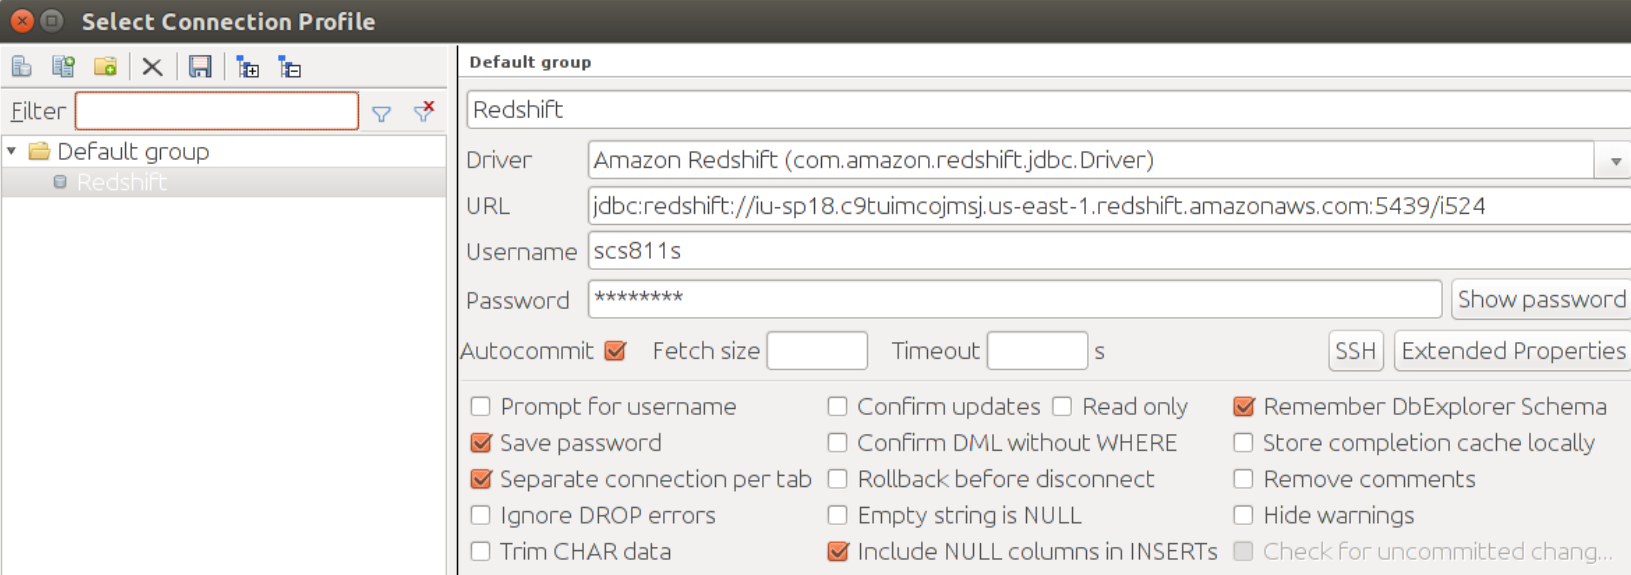
\includegraphics[width=\columnwidth]{images/sqlwkbench.png}
  \caption{SQL Workbench/J to Redshift}\label{f:sqlwkbench}
\end{figure}  

We used a variation of the code for the one-time run SQL queries we executed 
to create our RDS database, user and table. We also wanted our API user to 
only be able to run queries on the data in our Redshift table rather than 
being able to drop or create them. After setting up the Redshift environment 
for us to be able to interact with our Python code, our next step was import 
our data from S3 into Redshift. By using the Python library, psycopg2, we 
could interact with Redshift using the PostgreSQL Python 
functionality~\cite{hid-sp18-521-redshift-postgreSQL}. Using this library was 
very similar to the MySQL library, as we had to specify the database name, 
Redshift endpoint, port and user name in order to setup a connection and 
cursor object. We could then run a query that utilized the copy command to 
load our data from S3. This command required that we supply the Redshift table 
name, path to the CSV file located in S3, our access key info, and options to 
ignore the header row, remove the quotes from around the values and specify 
the comma delimiter in the source file as a comma. Executing this command 
within our API would then import the CSV file with our patient survey data on 
S3 directly into our Redshift 
table~\cite{hid-sp18-521-redshift-gettingstarted}. The Python code used to 
import the CSV data from S3 into Redshift is shown in 
Figure~\ref{f:redshiftload}. 

\begin{figure}[!ht]
\begin{verbatim}
redshift = psycopg2.connect(dbname= 'i524', 
host='iu-sp18.c9tuimcojmsj.us-east-1.redshift.amazonaws.com',
port='5439', 
user=redshift_user, 
password= redshift_password)

cur = redshift.cursor()

cur.execute(``COPY PatientSurveyData 
  FROM 's3://hid-sp18-521/PatientSurveyData.csv' ''
``ACCESS_KEY_ID ''' + k1 + 
``' SECRET_ACCESS_KEY ''' + k2 + ``' ''
``ignoreheader 1 ''
``removequotes ''
``delimiter ',';'')

return redshift.commit()
\end{verbatim}
\caption{Python code to insert S3 data into the Redshift table}
\label{f:redshiftload}
\end{figure} 

Then we wanted to provide the ability to query this data from within our code 
utilizing a SQL select statement. For our example use case, we coded a query 
to pull each state and their average star rating from the survey data to see 
how each state did overall at a high level. The execute function then 
submitted the query from our API and used the cursors fetchall function to 
store the query results returned back from Redshift into a variable. The 
Python code used to select data from the Redshift table is shown in 
Figure~\ref{f:redshiftquery}. 

\begin{figure}[!ht]
\begin{verbatim}
redshift = psycopg2.connect(dbname= 'i524', 
host='iu-sp18.c9tuimcojmsj.us-east-1.redshift.amazonaws.com',
port='5439', 
user=redshift_user, 
password=redshift_password)

cur = redshift.cursor()

cur.execute(``select location_state, 
avg(patient_survey_star_rating) 
from PatientSurveyData
where patient_survey_star_rating in (1,2,3,4,5) 
group by location_state 
order by location_state'')

sql = cur.fetchall()
redshift.commit()

return sql
\end{verbatim}	
\caption{Python code to select data from the Redshift table}
\label{f:redshiftquery}
\end{figure} 


Code to delete all data from the table was also implemented in order to 
promote reusability of our Redshift data loading if we ever had the need to 
reload the table with data from a new version of the S3 patient survey data 
file. This required just a simple delete statement to remove all rows from our 
Redshift table. The Python code used to delete data from the Redshift table 
is shown in Figure~\ref{f:redshiftdelete}. 

\begin{figure}[!ht]
\begin{verbatim}
redshift = psycopg2.connect(dbname= 'i524', 
host='iu-sp18.c9tuimcojmsj.us-east-1.redshift.amazonaws.com',
port='5439', 
user=redshift_user, 
password=redshift_password)

cur = redshift.cursor()

cur.execute(``DELETE FROM PatientSurveyData'')

return redshift.commit()
\end{verbatim}
\caption{Python code to delete data from the Redshift table}
\label{f:redshiftdelete}
\end{figure} 


\subsection{Athena}

The last AWS data related service we touched was Amazon Athena, one of the 
newer data services on the AWS platform. ``Amazon Athena is an interactive 
query service that allows users to analyze data directly in Amazon S3 using 
standard SQL~\cite{hid-sp18-521-whatisathena}.'' Its main use case is to allow 
the use of ad hoc SQL queries directly on files stored in S3 without having 
to ingest or aggregate this data in other data services in order to be able to 
perform analysis on it. The platform is serverless meaning there is no 
infrastructure to provision and scaling of query workload is handled 
automatically. Athena is able to query many different file formats and can 
handle querying structured, semi-structured and unstructured data. Before 
being able to run queries, metadata needed to be gathered on the files we 
would want to query in S3. ``In Athena, tables and databases are containers 
for the metadata definitions that define a schema for underlying source data. 
For each dataset, a table needs to exist in Athena. The metadata in the table 
tells Athena where the data is located in Amazon S3, and specifies the 
structure of the data, for example, column names, data types, and the name of 
the table. Databases are a logical grouping of tables, and also hold only 
metadata and schema information for a 
dataset~\cite{hid-sp18-521-whatisathena}.'' This meant we needed to first 
create a database to hold our metadata as well as a table structure that 
matches the patient survey data file we wanted to query on S3. We opted to use 
the internal Athena data catalog for our use case, but the option to use the 
AWS Glue Data Catalog also exists, which would allow Athena to automatically 
use the object metadata already collected and stored from other AWS data 
services that use AWS Glue~\cite{hid-sp18-521-whatisathena}.  

We started working with Athena by using the AWS Management Console 
functionality in order to gain an understand on how the service works. 
The main dashboard page for Athena consists of database and table information 
on the left side of the screen and an interactive query window in the middle. 
Athena has a default database in place for storing metadata, but we wanted to 
create our own. DDL queries run on Athena need to be submitted in 
HiveQL, which uses a simple create database command that other SQL based 
languages use and allowed us to create a new metadata database name i524. 
Since this would just be a one-time database creation, this functionality was 
not implemented into our APIs~\cite{hid-sp18-521-whatisathena}. 
Figure~\ref{f:athena} shows the Athena query editor which contains an input 
window where we could run our HiveQL code to create our metadata database
and run interactive queries as needed.

\begin{figure}[!ht]
  \centering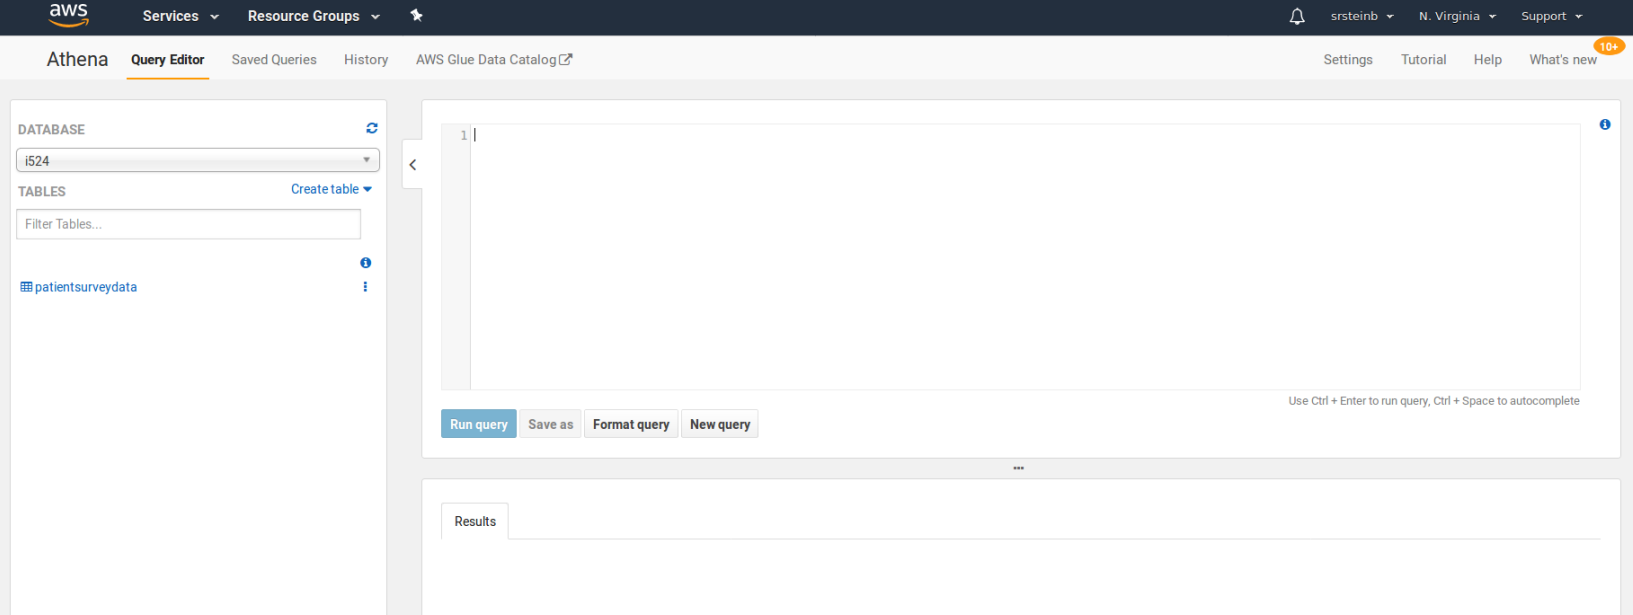
\includegraphics[width=\columnwidth]{images/athena.png}
  \caption{Athena query editor}\label{f:athena}
\end{figure}  

Next, we coded a create table DDL statement using HiveQL which would setup the 
metadata structure needed to be able to query the S3 file directly from 
Athena. Since we were creating the metadata table manually, the CSV file we 
wanted to use needed to exist in its own bucket separate from the rest of the 
files since the input parameters did not allow us to specify a direct S3 
file name to use. It only reqiored a file path which would then look for the 
file based on the source file type we indicated in the create table code. We 
used the resource API in Boto to establish a connection to Athena as we did 
for the other services we used in our APIs above. From there we could then use 
the start query execution method to run our DDL 
code~\cite{hid-sp18-521-boto-athena}. We opted to make this create table 
statement part of our API code in order to show how we could execute Athena 
queries programmatically. The create table command checks to see if the table 
already exists and if not, creates it. Additional properties about the source 
data file format, column separator, skipping the header row and quote 
identifiers were supplied, as well as the S3 bucket where the source file was 
located and the S3 bucket where we want the query results to be output 
to~\cite{hid-sp18-521-athena-gettingstarted}. The Python code used to import
CSV data from S3 into Athena is shown in Figure~\ref{f:athenainsert}. 

\begin{figure}[!ht]
\begin{verbatim}
athena = boto3.client('athena', region_name='us-east-1', aws_access_key_id=k1,
aws_secret_access_key=k2)

with smart_open.smart_open ('s3://' + k1 + ':' + k2 +'@hid-sp18-521/
athena-input/PatientSurveyData.csv', 'wb') 
as fout:
  for line in 
    smart_open.smart_open('https://data.medicare.gov/resource/
    rmgi-5fhi.csv'):
       response = fout.write(line + '\n')

response = athena.start_query_execution(QueryString=``CREATE EXTERNAL TABLE 
IF NOT EXISTS i524.PatientSurveyData (
...columns excluded from example, too many...
)
ROW FORMAT SERDE 
'org.apache.hadoop.hive.serde2.OpenCSVSerde' WITH SERDEPROPERTIES (
'separatorChar' = ',',
'quoteChar' = '\``'
)
STORED AS TEXTFILE 
LOCATION 's3://hid-sp18-521/athena-input'
TBLPROPERTIES (``skip.header.line.count''=``1'');'',
QueryExecutionContext={'Database': 'i524'}, 
ResultConfiguration={'OutputLocation': 's3://hid-sp18-521'})

return response
\end{verbatim}
\caption{Python code to insert S3 CSV data into Athena table}
\label{f:redshiftdelete}
\end{figure} 

For our example select query, we wanted to produce the records in the data set 
for a specific city that is specified by a user parameter in our API. Since 
we were not using the GUI to execute our select query, our results would need 
to be stored in a CSV output file in the folder parameter we provided during 
the create table statement. This functionality is by default and would then 
allow us to use the Athena query output in CSV format to send on to other data 
services for additional analysis if needed~\cite{hid-sp18-521-boto-athena}.  
The Python code used to query data from the Athena table is shown in
Figure~\ref{f:athenaquery}. 

\begin{figure}[!ht]
\begin{verbatim}
athena = boto3.client('athena', 
region_name='us-east-1', aws_access_key_id=k1, aws_secret_access_key=k2)

query = 'SELECT * FROM patientsurveydata WHERE city = \'%s\'' % (city)

response = athena.start_query_execution(QueryString=query,
   QueryExecutionContext={'Database': 'i524'}, 
   ResultConfiguration={'OutputLocation': 's3://hid-sp18-521'})

return response
\end{verbatim}
\caption{Python code to query the Athena table}
\label{f:athenaquery}
\end{figure} 

In order to be able to re-run our Athena test cases, we included a function 
to delete the Athena table so that we could repopulate it on demand as needed 
and used the same method start query execution that the other two Athena 
functions do in order to interact with the 
service~\cite{hid-sp18-521-boto-athena}. The Python code used to drop the  
Athena table is shown in Figure~\ref{f:athenadrop}. 

\begin{figure}[!ht]
\begin{verbatim}
athena = boto3.client('athena', region_name='us-east-1', aws_access_key_id=k1,
aws_secret_access_key=k2)

response = athena.start_query_execution(QueryString=
``DROP TABLE IF EXISTS PatientSurveyData'',
QueryExecutionContext={'Database': 'i524'}, 
ResultConfiguration={'OutputLocation': 's3://hid-sp18-521'})

return response
\end{verbatim}
\caption{Python code to drop the Athena table}
\label{f:athenadrop}
\end{figure} 


\section{Conclusion}

AWS offers cloud-based services for many different use cases and data 
platforms to meet a wide variety of user needs. By taking most of the backend 
administrative work out of managing and provisioning data platforms, we were 
able to spend the majority of our research time on interacting with each of 
the individual services through the AWS Management Console and AWS SDK for 
Python, called Boto. In the cases where exposing service setup to an end user 
didn't make sense, we learned how to perform configuration through the GUI so 
that we could then work programmatically with the data itself later on in our 
project. This was accomplished through the use of several Swagger APIs that 
called Python functions that used Boto functionality to be able to interact 
with the AWS resource and client APIs provided for each individual service we 
touched on. AWS provided stellar API documentation for Boto that allowed us to 
successfully write our Python code to extract, transform, load and query our 
Medicare patient survey data using six of AWS many data related services: S3, 
RDS, Data Pipeline, DynamoDB, Redshift and Athena.    

\begin{acks}
The authors would like to thank Dr.~Gregor~von~Laszewski for providing us
with an automated Latex document checker so that we could easily ensure
that our final paper was correctly formatted to proper Latex standards and 
layout.
\end{acks}

\bibliographystyle{ACM-Reference-Format}
\bibliography{report} 

